
%(BEGIN_QUESTION)
% Copyright 2005, Tony R. Kuphaldt, released under the Creative Commons Attribution License (v 1.0)
% This means you may do almost anything with this work of mine, so long as you give me proper credit

Some of the following transistor switch circuits are properly configured, and some are not.  Identify which of these circuits will function properly (i.e. turn on the load when the switch closes) and which of these circuits are mis-wired:

$$\includegraphics[width=15.5cm]{i01004x01.eps}$$

\underbar{file i01004}
%(END_QUESTION)





%(BEGIN_ANSWER)

Remember that a bipolar transistor requires current through the base-emitter junction in order to turn on, and thereby let load current pass between collector and emitter.

$$\includegraphics[width=15.5cm]{i01004x02.eps}$$

\vskip 10pt

Circuit \#3 is different from the other ``bad'' circuits.  While the other bad circuits' lamps do not energize at all, the lamp in circuit \#3 energizes weakly when the pushbutton switch is open (not actuated).  This is due to the fact that lamp current will naturally pass through the base-collector PN junction as though it were a simple diode, regardless of the switch's state.

%(END_ANSWER)





%(BEGIN_NOTES)


\vskip 20pt \vbox{\hrule \hbox{\strut \vrule{} {\bf Virtual Troubleshooting} \vrule} \hrule}

This question is a good candidate for a ``Virtual Troubleshooting'' exercise.  Presenting the diagram to students, you first imagine in your own mind a particular fault in the system.  Then, you present one or more symptoms of that fault (something noticeable by an operator or other user of the system).  Students then propose various diagnostic tests to perform on this system to identify the nature and location of the fault, as though they were technicians trying to troubleshoot the problem.  Your job is to tell them what the result(s) would be for each of the proposed diagnostic tests, documenting those results where all the students can see.

During and after the exercise, it is good to ask students follow-up questions such as:

\begin{itemize}
\item{} What does the result of the last diagnostic test tell you about the fault?
\item{} Suppose the results of the last diagnostic test were different.  What then would that result tell you about the fault?
\item{} Is the last diagnostic test the best one we could do?
\item{} What would be the ideal order of tests, to diagnose the problem in as few steps as possible?
\end{itemize}

%INDEX% Electronics review, transistor switch circuit (BJT)

%(END_NOTES)


